% main.tex -- four-page IEEE conference paper (Machine Learning and Data Mining, A.Y. 2026/27).
% Compile on Overleaf (pdfLaTeX + BibTeX); see paper/README.md.
% Convention: every sentence or table cell that carries a result number is followed by
% "% src: <file> <section>". Report files are outputs/reports/approved_<name>.md, written
% here as approved_<name>.md; design facts are cited to docs/APPROVED_PROPOSAL.md or to code.
\documentclass[conference]{IEEEtran}
\IEEEoverridecommandlockouts
\usepackage{cite}
\usepackage{amsmath,amssymb}
\usepackage{graphicx}
\usepackage{booktabs}
\usepackage{url}

\newcommand{\add}{\textsuperscript{\dag}}  % marks an addition beyond the approved text

\begin{document}

\title{Who Gets Flagged? A CRISP-DM Fairness Audit of\\ 30-Day Readmission Prediction}

\author{\IEEEauthorblockN{Uygar \c{C}atal}
\IEEEauthorblockA{University of Bologna, Cesena, Italy}}

\maketitle

\begin{abstract}
A hospital with limited follow-up capacity wants to flag the diabetic inpatients most likely to
be readmitted within 30 days, with equal errors across sex, age band and race. Following CRISP-DM,
we compare five classifiers on 98,470 encounters of the public Diabetes 130-US Hospitals data
under repeated patient-level cross-validation, flag the top $q$\,\% of each test fold, and audit
equalized odds with patient-bootstrap intervals and a permutation null. % src: approved_main.md header
The model with the highest ROC-AUC (random forest, 0.665; gradient boosting 0.664) ranks better
than chance, but no model passes the approved usability gate. % src: approved_main.md §1, §2
The clearest disparity is by age: the true-positive rate is 0.468 at ages 20--39 and 0.211 at
80+, mostly driven by better ranking of young patients, to which prior-use counts contribute much.
% src: approved_fairness.md §3.2; approved_sources.md §1, §5
Reweighing does not close the gap; the two post-processors that do achieve it by lowering
true-positive rates. % src: approved_mitigation.md §1-§3
Racial differences in recorded glucose results are largely, not wholly, a recording pattern. % src: approved_ordering.md §4
\end{abstract}

\begin{IEEEkeywords}
algorithmic fairness, equalized odds, hospital readmission, CRISP-DM, patient-level
cross-validation
\end{IEEEkeywords}

% ======================================================================================
\section{Introduction}

A hospital can follow up only a few discharged patients, so a readmission model is useful to it
as a \emph{ranking}: who gets the follow-up slots? The Diabetes 130-US Hospitals data were
released to study how HbA1c measurement relates to readmission~\cite{strack2014}. On them, a
patient-grouped gradient-boosting model predicts 30-day readmission with ROC-AUC 0.669, and its
balanced accuracy (0.622) matches the authors' estimated ceiling for the recorded
variables~\cite{chowdhury2026}. % src: chowdhury2026 (arXiv:2609.01909v1), "Cohort Results" and Table 1: patient-grouped GBDT AUROC 0.6692; best BA 0.6223 vs ceiling 0.6225
We therefore ask how the errors of such a model are distributed rather than push discrimination. Subgroup audits of these data exist~\cite{mateedulsatit2026,alzanbouri2024,abdelhay2026},
but none that we found measures fairness at a fixed intervention capacity, as resource-constrained
evaluation suggests~\cite{singh2023}; the closest judges a random forest at a 0.5 threshold on one
patient-level split~\cite{mateedulsatit2026}.
% src: mateedulsatit2026 (JMIR AI 5:e102146), Methods: conventional random forest, patient-level 80/20 split, prespecified probability threshold 0.50
Measurement matters too: whether a test is ordered carries information
of its own~\cite{agniel2018}, and unequal testing across groups can bias labels~\cite{chang2022}.

\emph{Question.} Can routinely collected admission data rank 30-day readmission risk well enough
to be used at a fixed capacity, are the errors equal across sex, age band and race, and if not,
where does the disparity come from and what does closing it cost? This is an individual assignment
(Option~2, CRISP-DM~\cite{shearer2000}) for the course \emph{Machine Learning and Data Mining},
University of Bologna, A.Y.~2026/27. It contributes a capacity-based
evaluation with a same-rule counterpart for every mitigation, a source analysis of the age gap, a
test-recording model and two honest negatives: no usable model, and levelling down.

% ======================================================================================
\section{Method following CRISP-DM}

The binding specification is the approved proposal, in the project repository with the code and
saved results (\url{https://github.com/uygarcatal6/readmission-fairness-audit}).
Choices it leaves open were fixed in writing before the results they affect, with one exception
marked below; additions beyond it are marked \add.

\subsection{Business understanding}
In each test fold the model flags the highest-risk $q$\,\% of encounters, where $q$ is the
readmission rate of the training fold (0.1144 overall). % src: approved_main.md header
This mimics a fixed follow-up capacity and reads no test label. The approved success criterion:
``A model counts as usable only if the lower confidence bound of (accuracy
$-$ 0.886) is above zero.'' The fairness goal is equalized odds~\cite{hardt2016}: equal
true- and false-positive rates (TPR, FPR) across sex, age band and race.

\subsection{Data understanding and preparation}
The raw data hold 101,766 inpatient encounters from 130 US hospitals (1999--2008) with 47
features~\cite{strack2014}. % src: docs/APPROVED_PROPOSAL.md §1
The weight column is about 97\,\% missing and is not used; payer code and medical specialty are
about 40\,\% and 49\,\% missing and keep ``unknown'' as a level. % src: data/profile.md:179-181 (weight 96.86 %, medical_specialty 49.08 %, payer_code 39.56 %); docs/APPROVED_PROPOSAL.md §1; adapters/diabetes_uci.py:78-82
We exclude encounters ending in death or hospice discharge, with unknown sex, with a missing primary
diagnosis, or in the two paediatric age bands, leaving 98,470 encounters from 69,303 patients, of
which 11,266 (0.1144) were readmitted within 30 days; the no-information rate (NIR) is 0.8856.
% src: approved_main.md header; approved_ordering.md §2; approved_fairness.md §1 (11,266 = 6,102 F + 5,164 M)
The target is readmission within 30 days versus everything else. The 23 model inputs, with the
primary ICD-9 diagnosis in nine groups, fall into six blocks: demographics, prior use
(visits in the year before), current stay, admission, diagnosis and diabetes care.
% src: approved_ordering.md §5; approved_sources.md block table
One-hot encoding (levels below 0.5\,\% of training rows pooled) and scaling are fitted on
training rows only. % src: readmission/preprocess.py:28, :31
The smallest group (Asian, 624 encounters, 65
readmitted) falls below 50 positives in a single test fold, so group metrics use each repeat's
pooled out-of-fold predictions. % src: approved_fairness.md §1; docs/APPROVED_PROPOSAL.md §3

\subsection{Modelling, validation and the usability gate}
The five approved models are a decision tree (pruning curves over depth and cost-complexity
$\alpha$), $k$-NN ($k$ from 1 to 1501), logistic regression, a random forest (300 trees, leaf size
5) and histogram gradient boosting, all from scikit-learn~\cite{pedregosa2011}; an MLP and bagging
are course extensions\add. % src: readmission/models.py:41-49
Outer validation is stratified group 5-fold cross-validation by patient, repeated 5 times.
% src: approved_main.md header
Depth and $k$ follow the one-standard-error rule on 5 inner patient-level folds: the simplest
candidate whose mean ROC-AUC is within one standard error of the best. Test folds are never used
for any choice. % src: readmission/evaluate.py:69 (n_inner = 5)
Confidence intervals come from 1000 patient-bootstrap draws, the same for all repeats; a point
estimate is the mean over repeats of the pooled out-of-fold metric.
% src: approved_main.md header
Sensitivity rules are $q = 5/10/20/30$\,\%, an inner-CV Youden threshold and a class-weighted model
at 0.5. With $m$ flagged, accuracy $-$ NIR $= (2\,\mathrm{TP}-m)/n$, so the gate needs a
positive predictive value (PPV) above 0.5. % src: approved_mitigation.md §3 note

\begin{table}[!t]
\caption{Approved models. ROC-AUC with 95\,\% patient-bootstrap CI; prevalence 0.114; BSS =
Brier skill score. Acc$-$NIR and EO age (equalized-odds difference by age band) at the capacity
rule (top $q$\,\%); every Acc$-$NIR upper 95\,\% bound is at most $-0.0539$, so no model passes the gate.}
% src: approved_main.md §1 (prevalence 0.114), §2 (highest upper bound -0.0539, rf)
\label{tab:models}
\centering\footnotesize\setlength{\tabcolsep}{3pt}
\begin{tabular}{@{}lccccc@{}}
\toprule
Model & ROC-AUC [95\,\% CI] & PR-AUC & BSS & Acc$-$NIR & EO age\\
\midrule
logreg & 0.653 [0.648, 0.659] & 0.205 & 0.034 & $-0.0607$ & 0.119\\ % src: approved_main.md §1, §2; approved_fairness.md §2
tree   & 0.648 [0.642, 0.654] & 0.202 & 0.035 & $-0.0600$ & 0.297\\ % src: approved_main.md §1, §2; approved_fairness.md §2
$k$-NN & 0.650 [0.644, 0.656] & 0.205 & 0.030 & $-0.0611$ & 0.128\\ % src: approved_main.md §1, §2; approved_fairness.md §2
rf     & \textbf{0.665} [0.659, 0.671] & 0.216 & 0.041 & $-0.0566$ & 0.257\\ % src: approved_main.md §1, §2; approved_fairness.md §2
hgb    & 0.664 [0.659, 0.670] & 0.214 & 0.041 & $-0.0571$ & 0.286\\ % src: approved_main.md §1, §2; approved_fairness.md §2
\bottomrule
\end{tabular}
\end{table}

\emph{Outcome.} The random forest (rf) has the highest ROC-AUC point estimate (hgb within its
CI) and ranks better than chance (Table~\ref{tab:models}), but at the capacity rule its TPR and PPV
are both 0.252 and accuracy $-$ NIR is $-0.0566$ [$-0.0594$, $-0.0539$]. % src: approved_main.md §1, §2
No model and no sensitivity rule passes the gate; the closest, rf at the top 5\,\%, reaches PPV
0.307 and accuracy $-$ NIR $-0.0193$ [$-0.0218$, $-0.0169$]. % src: approved_main.md §3
The one-SE rule picks tree depth 4 (20 of 25 splits; 5 otherwise) and $k = 1501$, the grid edge,
in all 25; a wider grid could only keep it or choose a larger (simpler) $k$. The MLP and
bagging extensions reach ROC-AUC 0.644. % src: approved_main.md §5, §6

\subsection{Fairness evaluation design}
\emph{Audit.} The primary model has the highest ROC-AUC, a rule fixed before fairness was seen. By sex, age band (20--39, 40--59, 60--79, 80+), race and sex~$\times$~age we report
TPR, FPR, PPV, selection rate and the equalized-odds (EO) difference, the larger of the TPR and FPR
ranges across groups. As approved: ``Groups with fewer than 50 positives (for TPR) or 50 negatives
(for FPR) are reported as insufficient, not dropped.'' PPV with fewer than 50 flagged is treated
alike\add. Race ``Unknown'' is a missing code and stays out of the race gap. A range is never below
zero, so we read it against a permutation null\add{} (200 patient-level shuffles of the attribute,
flags fixed) and signed pair differences\add. % src: approved_fairness.md §2
The paper leads with the attribute whose EO difference most exceeds its null\add{} (amended from
the approved ``largest baseline gap'' before the full results, because a range grows with the
number of small groups); both rules select age band. % src: approved_fairness.md header

\emph{Sources.} rf is refitted without one input block or sensitive attribute at a time; as a
weaker ranking can shrink a gap by itself, each arm is read against another seed\add{} and against
the full model losing the same ROC-AUC to random noise\add. A proxy model predicts each attribute
from the other inputs; ranking within groups is compared at the overall FPR\add.

\emph{Mitigations.} As approved, ``Each is compared with its unconstrained counterpart under the
same decision rule, so the reported accuracy cost comes from the mitigation and not from a change of
threshold.'' Reweighing uses Kamiran--Calders weights~\cite{kamiran2012}, compared with cell
balancing, at the capacity rule. fairlearn's ThresholdOptimizer~\cite{weerts2023} (EO constraint)
is fitted on a 20\,\% patient-level validation part of each training fold with balanced accuracy as
objective (the default, accuracy, flags at most 0.0023 of encounters); its counterpart is one
Youden threshold for everyone. % src: approved_mitigation.md §2, §3 note
Because that pair flags far more than $q$\,\%, we add EO post-processing at the capacity
rule\add{}~\cite{hardt2016}: randomised group thresholds with equal TPR and FPR while $q$\,\% are
flagged, compared with the same model flagging the same number. Levels with fewer than 50
validation positives are pooled for fitting; every mitigation is run for all three attributes.

\emph{Recording model.} A logistic regression relates ``HbA1c (or glucose) result recorded'', the
dataset's proxy for ``ordered'', to sex, age band, race and primary-diagnosis group, with
patient-clustered standard errors, Benjamini--Hochberg correction over the 16 sex, age and race
terms of both outcomes, and a replication on first encounters. A sensitivity fit adds an
``admission type unknown'' indicator\add, the one exception above: added after seeing the ordering
results, it is not tested. % src: approved_ordering.md header, §4

% ======================================================================================
\section{Results and insights}

\begin{figure}[!t]
\centering
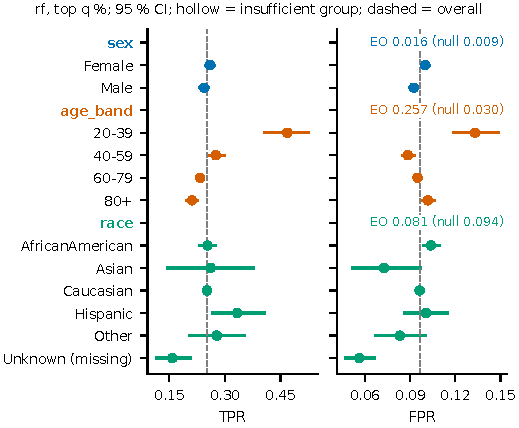
\includegraphics[width=0.9\columnwidth]{figures/fairness.pdf}
\caption{Group TPR (left) and FPR (right) of rf at the top $q$\,\% rule, 95\,\% CIs; dashed line
= overall rate; labels give each EO difference and its permutation-null mean.} % src: approved_fairness.md §2
\label{fig:fairness}
\end{figure}

\subsection{Fairness audit}
Age band leads: its EO difference is 0.257 [0.192, 0.320] against a null mean of 0.030
(permutation $p = 0.005$, the minimum for 200 shuffles; Fig.~\ref{fig:fairness}).
% src: approved_fairness.md §2; outputs/approved/fairness.json rf__topq age_band null p_value = 1/201
Young patients are flagged more often (selection rate 0.174 vs 0.107--0.115), with both a higher TPR
(0.468 vs 0.211 for 80+) and a higher FPR (0.133 vs 0.088--0.102). % src: approved_fairness.md §3.2
Sex shows 0.016 against a null of 0.009 ($p = 0.189$), and race 0.081, below its null mean of
0.094 ($p = 0.552$; 0.175 [0.109, 0.271] with the missing code included). % src: approved_fairness.md §2
Sex~$\times$~age (0.314) sharpens the age gap. % src: approved_fairness.md §2, §3.4
The gap is not a base-rate or calibration artefact: base rates by age lie within 0.101--0.125 and
observed minus predicted risk within $\pm 0.004$. % src: approved_fairness.md §1, §4
It depends on the model: logistic regression and $k$-NN show about half of it (0.119 and 0.128;
Table~\ref{tab:models}). % src: approved_fairness.md §2

\begin{figure}[!t]
\centering
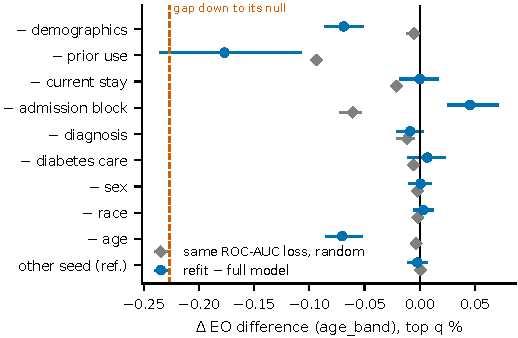
\includegraphics[width=\columnwidth]{figures/sources.pdf}
\caption{Change in the age-band EO difference when rf is refitted without one input block or
attribute (blue, 95\,\% CI) and when the full model loses the same ROC-AUC to noise (grey; min--max
of 5 draws). Dashed: change reaching the null.}
% src: approved_sources.md §1, §2
\label{fig:sources}
\end{figure}

\begin{table}[!t]
\caption{Mitigations on age band, rf (K\&C = Kamiran--Calders, TO = ThresholdOptimizer).
$\Delta$ = mitigated $-$ counterpart, same bootstrap draw. Counterparts: $^a$baseline and
$^b$same model, both flagging as many; $^c$one Youden threshold ($\Delta$ balanced accuracy).}
\label{tab:mitig}
\centering\footnotesize\setlength{\tabcolsep}{2pt}
\begin{tabular}{@{}lcccc@{}}
\toprule
Arm & EO & $\Delta$EO [95\,\% CI] & $\Delta$acc. & Flagged\\
\midrule
K\&C$^a$ & 0.257$\to$0.293 & $+0.036$ [0.026, 0.045] & $-0.0002$ & 0.114\\ % src: approved_mitigation.md §1, §5.1
Cell bal.$^a$ & 0.257$\to$0.146 & $-0.111$ [$-0.137$, $-0.087$] & $-0.0010$ & 0.114\\ % src: approved_mitigation.md §1, §5.1
EO at cap.\add$^b$ & 0.250$\to$0.018 & $-0.232$ [$-0.269$, $-0.146$] & $-0.0090$ & 0.115\\ % src: approved_mitigation.md §2
TO$^c$ & 0.188$\to$0.018 & $-0.170$ [$-0.181$, $-0.137$] & $-0.031$ & 0.365\\ % src: approved_mitigation.md §3
\bottomrule
\end{tabular}
\end{table}

\begin{figure}[!t]
\centering
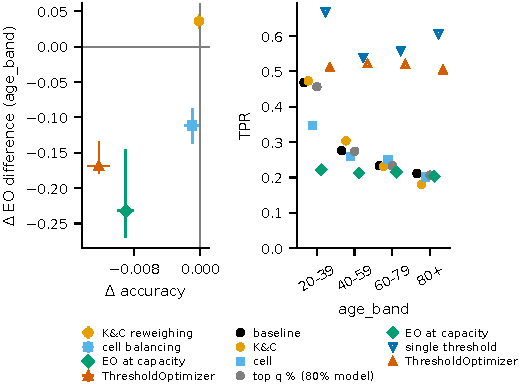
\includegraphics[width=\columnwidth]{figures/mitigation.pdf}
\caption{Left: $\Delta$EO (age band) against $\Delta$accuracy, each arm against the same model
flagging as many (TO: $\Delta$EO $-0.169$, $\Delta$acc. $-0.012$; Table~\ref{tab:mitig} gives TO against one threshold).
Right: TPR by age band; filled markers flag about $q$\,\%, hollow ones about 36\,\%: compare
within each set.}
% src: approved_mitigation.md §1-§3 (left panel; TO vs same-number twin = last two columns of §3), §5.1 (right panel; "compare within each set" note)
\label{fig:mitig}
\end{figure}

\subsection{Where the age gap comes from}
Removing the prior-use counts moves the gap most, from 0.257 to 0.080 ($\Delta$ $-0.177$
[$-0.236$, $-0.107$]), against 0.164 for the same ROC-AUC loss ($-0.045$) at random
(Fig.~\ref{fig:sources}). % src: approved_sources.md §1
The block contributes much of the gap, but removing it is no remedy: TPR for 20--39 falls from
0.468 to 0.245, while 80+ rises only from 0.211 to 0.230. % src: approved_sources.md §3
Removing age alone brings the gap to 0.187 ($\Delta$ $-0.070$ [$-0.086$, $-0.052$]; random
reference 0.254), yet the other inputs predict age band with ROC-AUC 0.773, so unawareness does not
remove the information. % src: approved_sources.md §2, §4
Removing sex or race leaves the gap unchanged; removing the admission block widens it (+0.046).
% src: approved_sources.md §1, §2
Most of it is ranking quality: within-group ROC-AUC falls from 0.755 (20--39) to 0.616 (80+); at
the overall FPR their TPRs would be 0.383 and 0.201, and the shared cut-off adds a further 0.085 to
the young. % src: approved_sources.md §5

\subsection{Mitigations}
Kamiran--Calders reweighing widens the age gap (+0.036, Table~\ref{tab:mitig}); it removes a
base-rate dependence that is small here. % src: approved_mitigation.md §1
Cell balancing narrows it by 0.111, but mostly as class balancing: balancing on race narrows the
age gap even more ($-0.124$). % src: approved_mitigation.md §1, §4
EO post-processing at capacity brings the gap to 0.018 at $\Delta$accuracy $-0.0090$ [$-0.0100$,
$-0.0081$], by lowering the TPR of 20--39 from 0.457 (same 80\,\% model; 0.468 for the full
model) to 0.222 while 80+ moves from 0.207 to 0.204 (Fig.~\ref{fig:mitig}).
% src: approved_mitigation.md §2, §5.1 (column "top q % (80 %)")
No age band's TPR rises: this is levelling down, not a fix. ThresholdOptimizer also reaches 0.018, but flags
0.365 of encounters and lowers every age TPR against its single threshold (20--39 0.668 to 0.510,
80+ 0.606 to 0.504). % src: approved_mitigation.md §3, §5.1
Among the sex-mitigation arms, none moves its EO difference by more than 0.022, every CI includes zero,
and none passes the usability gate. % src: approved_mitigation.md §1-§3, §7

\subsection{Test recording}
HbA1c results (0.166 of encounters) are recorded more often at ages 20--39 (odds ratio 1.60
[1.48, 1.73] vs 60--79) and for Hispanic patients (1.47 [1.32, 1.65]). % src: approved_ordering.md header, §2
Glucose results are recorded less often for African American (0.41 [0.35, 0.47]) and more often
for Hispanic patients (1.66 [1.31, 2.12]) than for Caucasian ones. % src: approved_ordering.md §2
Yet 79.7\,\% of glucose results come from the 10.2\,\% of encounters with an unknown admission type
(rate 0.406 vs 0.012). % src: approved_ordering.md §4
With that indicator the Hispanic excess is no longer distinguishable from one (1.10 [0.84, 1.43]),
while the African American deficit shrinks but remains (0.58 [0.50, 0.68]): the glucose race gaps
are largely, though not wholly, a recording pattern. The odds ratios describe who has a recorded
result and are not, on their own, evidence of unequal care. % src: approved_ordering.md header, §4
On first encounters, 15 of 16 tested terms keep their verdict. % src: approved_ordering.md §3

% ======================================================================================
\section{Conclusions}

A random forest ranks 30-day readmission risk better than chance, but no model, decision rule or
mitigation passes the approved usability gate (rf's PPV at capacity is 0.252; the gate needs more
than 0.5). % src: approved_main.md §2, §3; approved_mitigation.md §7
Its errors differ most by age: young patients are ranked better and flagged more; prior-use
counts and age itself contribute, while base rates and calibration do not explain the gap.
The glucose race differences are largely, not wholly, a recording pattern of the data source.
Reweighing does not close the age gap, and both post-processors that close it do so by lowering
TPRs; we do not call them a fix.

\emph{Limitations.} Hospital and period are not identified in the public file, so standard errors
are clustered by patient only. Bootstrap intervals are conditional on the fitted models, and randomised post-processing flags are fixed per
split. ``Result recorded'' is a proxy for ``test ordered'', and the admission-type sensitivity fit
is post hoc.

\emph{What a hospital should do (deployment).} It should not use the model as a stand-alone
classifier. If it allocates a fixed number of follow-ups by the ranking, it should report TPR by age
band beside overall performance and treat an equal-TPR constraint that lowers young patients' TPR as
a policy choice with a cost, not a fix. Better information on older patients' prior care and
complete recording of admission type and laboratory results may do more for equal errors than
post-processing (not tested here).

\section*{Use of AI assistants}
The author directed and designed the project: the topic and dataset within the course scope, the
research question, and a method built from a literature search and the author's earlier fairness
analysis, approved by the professor. The AI assistant Claude (Anthropic; Opus~5, Opus~5.5 and
Fable~5.1) did supporting analysis and technical work under this direction: code, runs,
feasibility and cost estimates, independent reviews and first drafts of the text. The author
reviewed every result and is responsible for the submission (full statement in the repository
README).

\bibliographystyle{IEEEtran}
\bibliography{references}

\end{document}
